% při kompilaci dokumentu LuaLaTeXem dojde k chybě, protože
% nedefinuje \pdfpagewidth a \pdfpageheight. 
% Balíček luatex85 to napravuje
\ifdefined\directlua
\RequirePackage{luatex85}
\fi

\documentclass{csbulletin}
% \usepackage[T1]{fontenc}
% \usepackage[utf8]{inputenc}
\usepackage{fontspec}
\setmainfont[Ligatures={TeX,Rare}]{Latin Modern Roman}
\selectlanguage{czech}
\usepackage{luavlna}
\usepackage[noautomatic]{responsive}
\usepackage[all]{nowidow}
\usepackage{csquotes}
\usepackage{linebreaker}

\usepackage{graphicx}
\usepackage{caption}
\usepackage{subcaption}
\usepackage{lipsum}


\usepackage[
  backend=biber,
  style=iso-numeric,
  sortlocale=cs,
  autolang=other,
  bibencoding=UTF8,
  mincitenames=2,
  maxcitenames=2,
]{biblatex}
\addbibresource{responsive.bib}
\usepackage[
  implicit=false,
  hidelinks,
]{hyperref}


\newcommand\balicek[1]{\textit{#1}}
\newcommand\program[1]{#1}


\newcommand\printsize[1]{\csname #1\endcsname\par\noindent Sample \par}
\newcommand\showscale[2][.5\textwidth]{%
      % \setsizes[38]{25}
      \printsize{huge}
      \printsize{LARGE}
      \printsize{Large}
      \printsize{large}
      \hrule
      \printsize{normalsize}
      \hrule
      \printsize{small}
      \printsize{footnotesize}
}


\begin{document}

\title{Responzivní design s \LaTeX em}
\EnglishTitle{Responsive Design with \LaTeX}
\author{Michal Hoftich}
\podpis{Michal Hoftich, \url{michal.h21@gmail.com}}
\maketitle

\begin{abstract}
Tento článek se zaměřuje na použití metod responzivního designu pro zobrazení
webových stránek na zařízeních s různou velikostí displejů, jako jsou mobilní
telefony, tablety, velké monitory a tiskárny. Tyto metody umožňují optimalizaci
čitelnosti dokumentu na všech zařízeních pomocí použití různých velikostí
písma, jednotlivých prvků na stránce a okrajů.

Představíme způsob, jak lze podobné funkcionality dosáhnout
pomocí \LaTeX u. Konkrétně se zaměřuje na využití Lua\LaTeX u pro automatizovanou
sazbu s pomocí balíčků \balicek{Responsive}\cite{responsive} pro nastavení velikosti písma a řádkového prokladu
podle velikosti stránky, \balicek{Luavlna} \cite{luavlna} pro zamezení výskytu jednopísmenných předložek
na koncích řádků, \balicek{Lua-widow-control}  \cite{lua-widow-control} pro omezení osamocených řádků na koncích a
začátcích stránek a \balicek{Linebreaker} \cite{linebreaker}, který brání přetečení řádků.

Díky těmto metodám lze použít jeden zdrojový dokument pro různé výstupy, jako
jsou tiskové verze, čtečky e-knih a webové stránky, a dosáhnout optimálního
zobrazení dokumentu na všech zařízeních.
\end{abstract}
\klicovaslova: automatická sazba, responzivní design, Lua\LaTeX


\section{Úvod}

Před časem jsem si pořídil čtečku elektronických knih, ale i přesto většinu
textů čtu z obrazovky svého PC, protože pochází z webových zdrojů, především 
různých blogů. To má za důsledek několik problémů, například únavu očí, bolesti zad
z příliš dlouhého sezení na židli, nemluvě o zbytečně spotřebované elektrické
energii. Napadlo mě tedy, že bych bych si delší články ukládal pro pozdější
přečtení na čtečce. K tomuto účelu samozřejmě existuje řada aplikací, ale 
já se rozhodl vytvořit si vlastní, kterou si přizpůsobím přesně svým potřebám
a preferencím. Další motivací je možnost naučit se něco nového a vytvořit
balíčky, které budou užitečné i pro další uživatele \TeX u. 

Protože díky Lua\TeX u je v \TeX ových distribucích dostupný programovací jazyk 
Lua, využil jsem ho pro vytvoření svého projektu \program{Rmodepdf} \cite{rmodepdf}.
Ten využívá balíček \balicek{LuaXML} \cite{luaxml} pro 
transformaci HTML na \TeX{} a příkazy \program{Curl} pro stažení stránky, \program{Tidy} 
pro opravu chyb v HTML a \program{Rdrview} \cite{rdrview}, který odstraní
ze stránky navigační prvky, reklamy a jiné rušivé elementy. \program{Rdrview} 
tak funguje podobně jako mód zobrazení čtečky v prohlížeči \program{Firefox}
(ilustrováno v obrázku~\ref{fig:readermode}).

V následujícím textu se však nezaměřím na samotný \program{Rmodepdf}.
Myslím, že pro čtenáře bude užitečnější popis metod pro automatickou sazbu,
které lze využít i pro jiné účely, například při konverzi z dokumentů ve formátu MS Word, 
nebo elektronických knih ve formátu Epub. Zde nevyužijeme funkci
odstraňování navigačních prvků ze stránky, ale můžeme zde využít
přizpůsobení velikosti písma velikosti stránky nebo automatické řešení
typografických problémů či špatně zalomených řádků.

\begin{figure}[htbp]

  \centering
  \caption{Ukázka použití režimu \emph{zobrazení čtečky} v prohlížeči \program{Firefox}}
  \label{fig:readermode}

  \begin{subfigure}[t]{0.45\textwidth}
    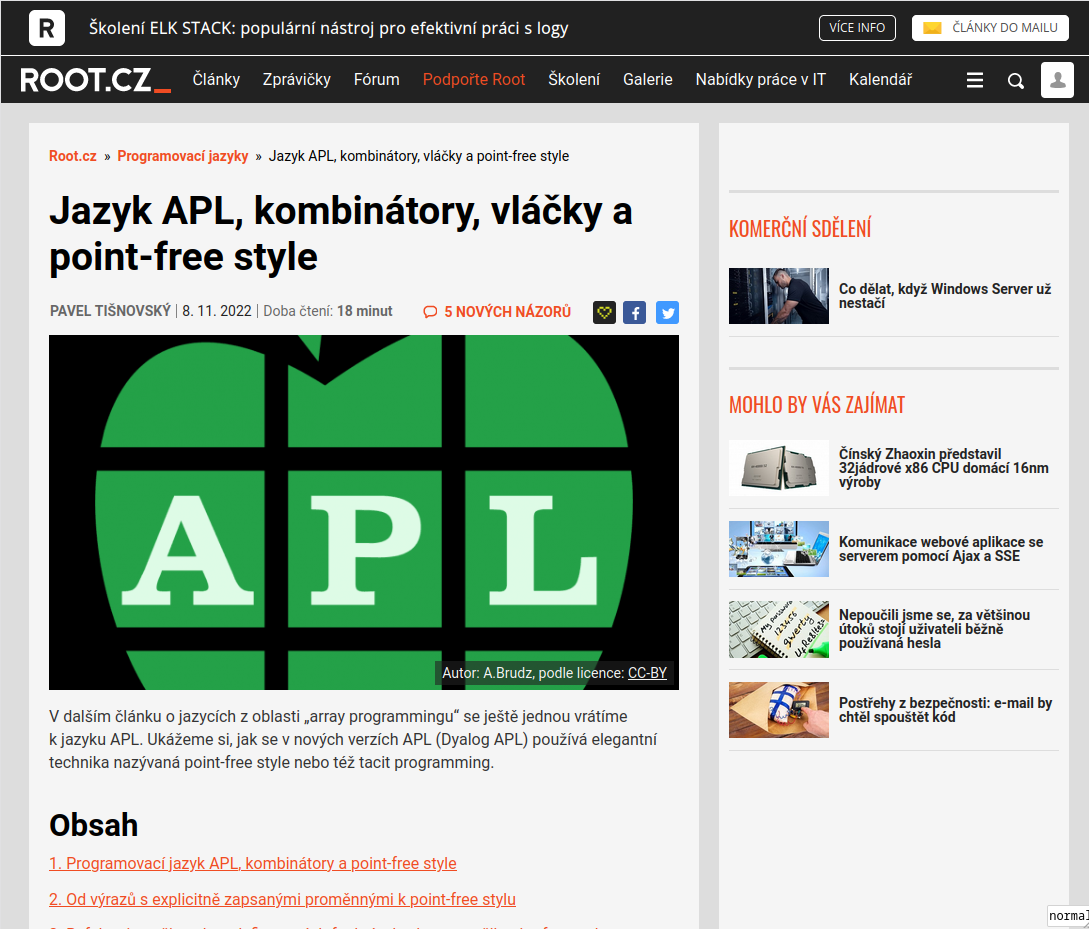
\includegraphics[width=\textwidth]{img/root-balast.png}
    \caption{Stránka s ovládacími prvky a reklamami}
  \end{subfigure}
  \hfill
  \begin{subfigure}[t]{0.45\textwidth}
    \includegraphics[width=\textwidth]{img/root-čtečka.png}
    \caption{Stránka v zobrazení čtečky}
  \end{subfigure}
\end{figure}

% \section{Jak s pomocí \LaTeX u převést webovou stránku na PDF}

% % https://github.com/eafer/rdrview

% \begin{verbatim}
% $ rdrview -H <url> | pandoc -f html -t latex -V lang=cs \
%   --template template.tex output.html > output.tex
% \end{verbatim}

\section{Responzivní design}

Prvním problémem, který jsem řešil, bylo nastavení správné velikosti písma 
z hlediska čitelnosti. 
Výchozí velikost písma v \LaTeX u je 10 bodů, bez ohledu na velikost
stránky. To je vhodná velikost pro stránku formátu A5. Pro formát
A4 by měla být větší, naopak pro menší displeje čteček a mobilních
telefonů může být menší. Stejný problém řeší webové prohlížeče,
které musí zobrazit text jak na velkých monitorech PC, tak na
menších displejích notebooků, tabletů a mobilních telefonů. 
Řešením, který používají, je \textit{responzivní design}.



Responzivní design je způsob návrhu webových stránek, který umožňuje
pružné a dynamické přizpůsobení vzhledu a uspořádání obsahu stránky
různým zobrazovacím zařízením. Jedním z klíčových prvků responzivního
designu je flexibilní struktura, která umožňuje přizpůsobit velikost
prvků na stránce zobrazovacímu zařízení.

Dalším důležitým prvkem jsou media queries, které umožňují definovat
pravidla, která se aplikují na základě vlastností zobrazovacího
zařízení, jako je velikost displeje, druh displeje, atd. Díky těmto
vlastnostem může stejný kód stránky být dobře zobrazen jak na velkém
monitoru, tak na mobilních zařízeních. Ukázku reálného využití 
můžete vidět na obrázku~\ref{fig:responzivni}.


\begin{figure}[htbp]
  \caption{Ukázka zobrazení webové stránky s využitím responzivního designu}
  \label{fig:responzivni}
\begin{subfigure}[t]{0.74\textwidth}
    
\includegraphics[width=\textwidth]{img/pedf-web-big.png}
    \caption{Ukázka stránky na velkém monitoru}
\end{subfigure}
\hfill
\begin{subfigure}[t]{0.24\textwidth}
    \includegraphics[width=\textwidth]{img/pedf-web-small.png}
    \caption{Ukázka stránky na malém displeji}
\end{subfigure}
\end{figure}

Můj nový balíček \balicek{Responsive} se těmito zásadami inspiroval. 
Jeho hlavní funkcí je nastavení velikosti písma podle velikosti stránky
a přibližného počtu znaků, které by se měly vejít na stránku. 
Dále nastavuje typografickou stupnici (ovlivňuje velikost písma například 
u nadpisů nebo poznámek pod čarou), písmovou osnovu a podporuje
jednoduchou verzi media queries.

\subsection{Nastavení balíčku \balicek{Responsive}}

\balicek{Responsive} automaticky nastavuje velikost písma, řádkový proklad
a typografickou stupnici na začátku dokumentu. Výchozí hodnoty můžeme změnit
pomocí voleb balíčku, nebo příkazem \verb|\ResponsiveSetup|, který můžeme 
využít i v dokumentu, například pro lokální změny nastavení písma. 

Hlavní volby balíčku jsou tyto:

\begin{description}
  \item[noautomatic] – nenastavovat velikost písma automaticky na začátku dokumentu
  \item[characters] – počet znaků při automatickém nastavení velikosti písma
  \item[scale] –  typografická stupnice použitá pro velikosti řezů písma
  \item[lineratio] – poměr využitý při výpočtu řádkového prokladu
\end{description}

\subsection{Základní velikost písma}

Velikost písma můžeme nastavit pomocí příkazu \verb|\setsizes{<počet znaků na|\allowbreak\verb|řádek>}|. 
\balicek{Responsive} se snaží nastavit velikost písma tak, aby na řádku byl v průměru
požadovaný počet znaků. Skutečný počet znaků samozřejmě záleží na použitém textu, ve 
skutečnosti bývá mírně vyšší.

Pokud neuvedeme počet znaků, použije se hodnota volby \texttt{characters}.
Následující příklad využívá právě nastavení této volby. Obrázek~\ref{fig:fontsize} 
ukazuje, jak se stejný text může v daném rámci zobrazit rozdílně v závislosti na
nastavených volbách.

\begin{verbatim}
\begin{minipage}{5cm}
\ResponsiveSetup{characters=55}
\setsizes{}

\lipsum[1]

\end{minipage}}
\end{verbatim}
 
\begin{figure}
  \caption{Rozdíl velikosti písma v závislosti na počtu znaků}
  \label{fig:fontsize}
  \begin{subfigure}[t]{0.45\textwidth}
\fbox{%
\begin{minipage}{5cm}
\ResponsiveSetup{characters=55}
\setsizes{}

\lipsum[1]

\end{minipage}}
\caption{\texttt{characters=55}}
\end{subfigure}
\begin{subfigure}[t]{0.45\textwidth}
\fbox{%
\begin{minipage}{5cm}
\ResponsiveSetup{lineratio=38,characters=25}
\setsizes{}

Lorem ipsum dolor sit amet,
consectetuer adipiscing elit.
Ut purus elit, vestibulum ut,
placerat ac, adipiscing vitae,
felis. Curabitur dictum gravida 
mauris. Nam arcu libero, nonummy 
eget, consectetuer id, vulputate 
a, magna. Donec vehicula augue eu neque.

\end{minipage}}
\caption{\texttt{characters=25, lineratio=38}}
\end{subfigure}
\end{figure}

\subsection{Řádkový proklad}

\begin{figure}
  \begin{subfigure}[b]{0.45\textwidth}
\fbox{%
\begin{minipage}{5cm}
\ResponsiveSetup{lineratio=38}
\setsizes{65}

\lipsum[1]

\end{minipage}}
\caption{lineratio=38}
\end{subfigure}
\begin{subfigure}[b]{0.45\textwidth}
\fbox{%
\begin{minipage}{5cm}
\ResponsiveSetup{lineratio=34}
\setsizes{65}

\lipsum[1]

\end{minipage}}
\caption{lineratio=34}
\end{subfigure}
\end{figure}

\subsection{Typografická stupnice}


Klasická typografická stupnice je soubor velikostí písma, které jsou vizuálně v
harmonii. Podobně jako hudebník vybírá noty z hudební stupnice, typograf si
vybírá velikosti z typografické stupnice.  
\cite{mortensen}


\begin{figure}
  \caption{Ukázka typografických stupnic (výchozí velikost písma je zvýrazněna linkami)}
  \label{fig:stupnice}
  \begin{subfigure}[b]{0.45\textwidth}
\fbox{%
\begin{minipage}{5cm}
\setsizes{45}

\showscale{}

\end{minipage}}
\caption{Výchozí stupnice (pentatonická)}
\end{subfigure}
\begin{subfigure}[b]{0.45\textwidth}
\begin{verbatim}
\ResponsiveSetup{scale=golden}
\end{verbatim}
\fbox{%
\begin{minipage}{5cm}
\ResponsiveSetup{scale=golden}
\setsizes{45}

\showscale

\end{minipage}}
\caption{Stupnice založená na zlatém řezu}
\end{subfigure}
\end{figure}

\printbibliography

\begin{summary}
  This article focuses on the use of responsive design techniques to display
  web pages on devices with different display sizes, such as mobile phones,
  tablets, large monitors and printers. These methods allow optimizing the
  readability of a document on all devices by using different font sizes,
  individual page elements, and margins.

  We present how similar functionality can be achieved using \LaTeX.
  Specifically, it focuses on the use of Lua\LaTeX{} for automated typesetting,
  using packages \balicek{Responsive} for setting font size and line spacing according to page size,
  \balicek{Luavlna} to prevent the occurrence of
  single-letter prepositions at line breaks, \balicek{Lua-widow-control} to
  reduce orphan lines at page breaks and page starts, and \balicek{Linebreaker}
  to prevent line overflow.

  With these methods, a single source document can be used for different
  outputs, such as print versions, e-book readers, and web pages, and achieve
  optimal document display on all devices.

\keywords: automatic typesetting, responsive design, Lua\LaTeX
\end{summary}
\end{document}
